\documentclass[tikz,border=10mm]{standalone}
\usetikzlibrary{calc}


% This file generates a checkerboard pattern
% The defs below define its size:

\def\xw{3}
\def\yw{2}
\def\dist{20.0mm}

\begin{document}
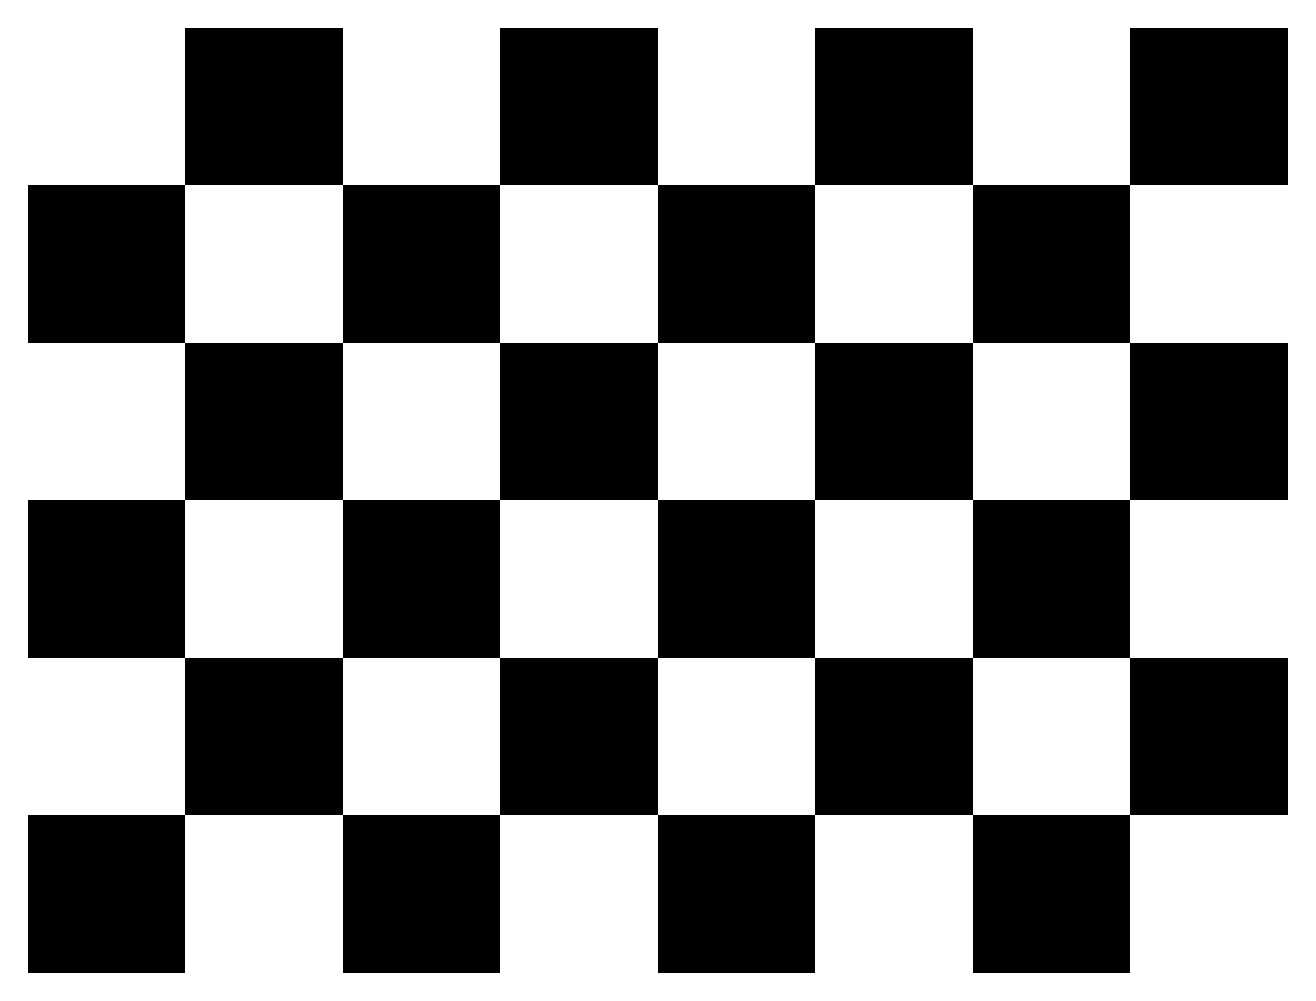
\begin{tikzpicture}[scale=1]





\foreach \c in {0,...,\yw}{
    \foreach \b in {0,...,\xw}{
       \fill[black] (2*\b*\dist-\dist,2*\c*\dist-\dist) rectangle (2*\b*\dist,2*\c*\dist);
       \fill[black] (2*\b*\dist,2*\c*\dist) rectangle (2*\b*\dist+\dist,2*\c*\dist+\dist);
    }

}


\end{tikzpicture}
\end{document}
